\documentclass[9pt,aspectratio=169]{beamer} %8pt for font size
%\documentclass[handout]{beamer}
%\usetheme{jambro}\usefonttheme[onlymath]{serif}
\usepackage[utf8]{inputenc}
\usepackage{appendix}
\setbeamertemplate{footline}[frame number]

\usepackage{amsmath}
\usepackage{graphicx}
\usepackage{subfig} % Manipulation and reference of small or sub figures and tables
\usepackage{tikz}
\usepackage{hyperref}
\usepackage{caption}
\usepackage{blkarray}
\usepackage{pgfplots}
\pgfplotsset{compat = newest}
\usetikzlibrary{positioning, arrows.meta}
\usepgfplotslibrary{fillbetween}
\usepackage{appendixnumberbeamer}
\usepackage{mathtools, stackengine}
\usepackage{amsfonts}
\usepackage{textpos}
\usepackage[makeroom]{cancel}
\usepackage[normalem]{ulem}  % For strikethrough

%\setbeamercovered{again covered={\opaqueness<1->{15}}, dynamic}
\setbeamercovered{transparent=0}
\definecolor{carandache}{RGB}{218,165,32}   % black for underlying
\usepackage[absolute,overlay]{textpos}

%These provide extra spacing and then correct the frame title back up
\renewcommand{\baselinestretch}{1.5}
%\setstretch{2.0}

\addtobeamertemplate{frametitle}{\vspace*{-0.2cm}}{\vspace*{0.1cm}}

\usetikzlibrary{decorations.pathreplacing,calc}
% For text blocks (like "Risk-neutral firm...")
\newcommand{\ntikzmark}[2]{%
  \tikz[remember picture,baseline=(#1.base)]{\node[inner sep=0pt,outer sep=0pt] (#1) {#2};}%
}

% For inline nodes (like "job", "convenient")
\newcommand{\innode}[2]{%
  \tikz[remember picture,baseline=(#1.base),inner sep=0pt,outer sep=0pt]{\node[anchor=base] (#1) {#2};}%
}
\usetikzlibrary{calc} %I HAD TO CORRECT THE BRACES MANUALLY
\newcommand{\makebrace}[3]{%
    \begin{tikzpicture}[overlay, remember picture]
        \draw [decoration={brace,amplitude=0.5em},decorate]
        let \p1=(#1), \p2=(#2) in
        ({max(\x1,\x2)+10em}, {\y1+0.8em}) -- node[right=0.6em] {#3} ({max(\x1,\x2)+10em}, {\y2});
    \end{tikzpicture}
}


\tikzset{
  baseline=(current bounding box.center), % Default baseline alignment
  every node/.style={anchor=base, inner sep=0pt, outer sep=0pt, font=\normalfont} % Reset node styles
}

\begin{document}



\makeatletter
\let\save@measuring@true\measuring@true
\def\measuring@true{%
  \save@measuring@true
  \def\beamer@sortzero##1{\beamer@ifnextcharospec{\beamer@sortzeroread{##1}}{}}%
  \def\beamer@sortzeroread##1<##2>{}%
  \def\beamer@finalnospec{}%
}
\makeatother


\title{Wage and Layoffs Risk Across Tenure}
\author{Andrei Zaloilo \\ Toulouse School of Economics}

\date{March 2025}

\maketitle

\begin{frame}{Introduction}
\hypertarget{Intro}
Young workers are subject to higher than average aggregate earnings risk \textcolor{gray}{(Guvenen et al. 2017)} \\
\begin{itemize}
    \item Firm-level risk: Higher layoff rate, higher layoff passthrough, lower wage passthrough
    \vspace{5pt}
    \item {BUT} most of the heterogeneity is due to differences in \textcolor{red}{tenure} \hyperlink{MotivEv}{\beamerbutton{Evidence}}
\end{itemize}
\vspace{10pt}
\textbf{This paper:} A framework of workforce management and wage/layoff trade-off \\
\begin{itemize}
    \item Long-term state- and tenure-contingent contingent contracts specifying wages and layoff risk
    \vspace{5pt}
    \item Reconcile the wage/layoff passthrough heterogeneity across tenure
    \vspace{5pt}
    \item Consistent with 
    \begin{itemize}
        \item Cross-firm size heterogeneity in wage/layoff passthrough (French admin data)
        \item Large scale survey+admin evidence \textcolor{gray}{(Bertheau et al. 2024)}
        \begin{itemize}
            \item "Firms that express opportunistic layoffs are less likely to implement wage cuts"
        \end{itemize}
    \end{itemize}
    %\vspace{5pt}
    %\item Adverse implications of labor policies: hiring subsidies \textcolor{red} {raise} layoff risk for juniors
\end{itemize}

\end{frame}

\begin{frame}{Model Ingredients} %AUGMENT THIS LATER WITH RESULTS! THAT OR MOVE MECHANISM TO ANOTHER SLIDE AND DROP STUFF THERE
\textbf{Theory}: layoffs give better control (rather than wage cuts)  over \textcolor{red}{which worker leaves}
\begin{itemize}
    \item \textcolor{blue}{Heterogeneous match quality}
    %\item \underline{Asymmetric information}: only firm knows, who is productive $\rightarrow$ can't set quality-dependent wages
\vspace{5pt}    
    \item \textcolor{blue}{No quality-dependent wages}: can't use wages to rid of unproductive workers
\vspace{5pt}
    \item \textcolor{blue}{Decreasing returns to scale}: replace unproductive workers instead of scaling up
\end{itemize}
\vspace{5pt}
Wage setting - \textcolor{blue}{Dynamic contracting}: state- and tenure-contingent wages and layoffs

%%\pause
\vspace{15pt}
%Introduce dynamic contracting framework into a multi-worker firm with heterog quality \\
    \textbf{Mechanism:}
\begin{itemize}
    \item Firms want to optimize both quantity and \textcolor{red}{quality} of workers
    \item Newly hired workers on average less productive and cheaper to lay off
    \item In low prod periods, firms fire juniors to reduce payroll and raise worker quality
        \begin{itemize}
            \item Remaining juniors, now of higher avg quality, take smaller wage cuts than seniors
        \end{itemize}
\end{itemize}
%Policy prediction: Large firms fire more workers, mainly juniors, small firms lower wages
\end{frame}

\begin{frame}{Physical Environment}
Discrete time, measure of workers and firms \\
\vspace{10pt}
\textbf{Production}: \\
Unemployed workers produce $b$ \\

Firms employ a measure $n$ of workers to produce
    \begin{itemize}
        \item Stochastic productivity, $y$ - stochastic shifter
        \vspace{5pt}
        \item The firm-worker match can be of high quality ($p=q_0$) or of low quality
        \vspace{5pt}
        \item Only the firm knows the match quality, $z$ - proportion of high q matches
        \vspace{5pt}
        \item Firm produces $yF(g(z)n)$ - DRS
        \end{itemize}
\vspace{10pt}
Incumbent firms have to pay $\kappa_f$ every period, new firms can pay $\kappa_e$ to open
\end{frame}

\begin{frame}{Market Environment}
\hypertarget{PE}
Firms may lay off proportion $s$ of employed workers and hire $\tilde{n}$ new workers of avg quality $z_0$\\
\vspace{10pt}
Workers, both unemployed and employed, search for a job \\
\vspace{10pt}
Search is directed:
\begin{itemize}
    \item Workers decide in which submarket to search
    \item Free-entry of firms, incumbent firms decide where to post vacancies  \hyperlink{Block Recur}{\beamerbutton{Block Recursivity}} 
\hyperlink{GE}{\beamerbutton{GE}}
\end{itemize}

\vspace{20pt}
    \begin{figure}
        \centering
\begin{tikzpicture}[node distance=2mm]
  \draw[->] (0,0) to  (10,0);
    \filldraw[black] (0,0) circle (2pt);
  \node[below, black] at (0,-2mm) {t};
    \filldraw[black] (9,0) circle (2pt);
  \node[below, black] at (9,-2mm) {t+1};
  \foreach \x/\q in {2/,4/,6/,8/}{
    \draw[line width=1pt, black] (\x,-2mm) node[below, black](a\x){\q} -- (\x,2mm);
}
\node [below=of a2, align=center, minimum width=1in, minimum height=1cm] {$F(g(z)n)$,$w$ \\ Production and Wage };
\node [above=of a4, align=center, minimum width=1in, minimum height=1cm] {Firm Layoffs $s$};
\node [below=of a6, align=center, minimum width=1in, minimum height=1cm] {Hiring $\tilde{n}$ \\ Worker Search $p(\theta)$};
\node [above=of a8, align=center, minimum width=1in, minimum height=1cm] {Prod Shock $z_{t+1}|z_t$};
\end{tikzpicture}
\caption{Within-period time line} \label{fig:M1}
\end{figure}
\end{frame}

\begin{frame}{Contracting Framework}
\hypertarget{Contracting}
%\begin{itemize}
  \onslide<1-2>{
  \textbf{Dynamic Contracting}: history-contingent wages and layoff risk, subject to ex-ante worker value \\
  \vspace{5pt}
    \ntikzmark{L}{Risk-neutral firm with stochastic productivity $y$} \\  
    \ntikzmark{O}{Risk-averse worker} \\

    \vspace{5pt}
    Limited commitment: worker moves to another job or into unemployment if \innode{node1}{convenient} \\
    \vspace{5pt}
    \textbf{Recursive Formulation}: $\mathcal{C} \equiv \big\{w, s, \{v' \}_{y'} \big\}$; \ \ $v$: promised utility 
    % Arrows
    \begin{tikzpicture}[remember picture,overlay]
      \draw[->,blue] (node1.north east) to[bend right] ++(0.3,0.3) node[brick,anchor=west] {\small\hand Incentive provision};
    \end{tikzpicture}
    \makebrace{L}{O}{{\small{\hand \textcolor{blue}{Insurance provision}}}}
    }
    \\ \vspace{10pt}
    
\onslide<2>{ Merged with \textbf{firm dynamics}: contracts connected  \\
\begin{itemize}
    \item A Limited Tenure Approximation: differentiate workers by tenure, up to $K$ \innode{node3}{steps} \hyperlink{Wage growth}{\beamerbutton{Wage growth in the data}}
    \vspace{5pt}
    \item Junior workers always hired at the same value $v_0$
\end{itemize}
\vspace{10pt}
\textbf{Match heterogeneity}: 2 prod types, keep track of avg quality
    \begin{itemize}
        \item Workers don't know their quality, compensated for ex-ante layoff risk
        \item \textcolor{red}{Can't} set quality-dependent wages: only layoffs affect quality
    \end{itemize}
    \begin{tikzpicture}[tpstyle,remember picture,overlay]
		\draw[arrow,->,red] ([yshift=1pt]node3.north east) to[bend right] +(0.0,+0.3) node[red,anchor=east] {\small{\hand Tenure-specific contract $\mathcal{C}_k$}};
    \end{tikzpicture}	
}

\end{frame}

\begin{frame}[noframenumbering]{Firm Problem}

%\textcolor{blue}{Still to do:} add k's to some extra places, figure out the exact timing, decide how to color size (maybe separately from tenure stuff?) (maybe have them all separate from each other?)\\
Choose wages $w$, \only<4->{\textcolor{red}{quality-contingent}} separations $s$, future promise $v'_{y'}$ \only<2-2>{\textcolor{black}{for each worker $i$}} \only<3->{\textcolor{blue}{at each tenure level}} to maximize:
    \[
    J(y,\only<3->{\textcolor{blue}{\{}}\only<2->{\textcolor{black}{n}}\only<3->{\textcolor{blue}{_k\}}}\only<2->{,}\only<3->{\textcolor{blue}{\{}}\only<2-2>{\textcolor{black}{P(}}v\only<2-2>{\textcolor{black}{_i)}}\only<3->{_{{\textcolor{blue}{k}}}\textcolor{blue}{\}}}\only<4->{,\textcolor{red}{\{z_k\}}})=
    %Max
    \max_{v'_{y'\only<2->{,\only<2-2>{\textcolor{black}{i}}\only<3->{\textcolor{blue}{k}}}},w_{\only<2-2>{\textcolor{black}{i}}\only<3->{\textcolor{blue}{k}}},s_{\only<2-2>{\textcolor{black}{i}}\only<3->{\textcolor{blue}{k}}}\only<2->{,\textcolor{black}{\tilde{n}}}} 
    %Production
    \underbrace{y\only<2->{\textcolor{black}{F(}}\only<3->{\textcolor{blue}{\sum_k}\only<4->{\textcolor{red}{g(z_k)}}} \only<2->{\textcolor{black}{n}}\only<3->{\textcolor{blue}{_k}} \only<2->{\textcolor{black}{)}}}_{\text{\only<2->{\textcolor{black}{DRS}} Production}}-
    %Wage
    \underbrace{\only<3->{\textcolor{blue}{\sum_k}} \only<2-2>{\textcolor{black}{\int}}w\only<2-2>{\textcolor{black}{_idP(v_i)}}\only<3->{\textcolor{blue}{_k}}
    \only<3->{\textcolor{black}{n}}\only<3->{\textcolor{blue}{_k}}}_{\text{Payroll}}
    \only<2->{-\underbrace{\textcolor{black}{\frac{c}{q}\tilde{n}}}_{\text{Hiring}}}
    %Expectation
    \only<2->{-\kappa_f}+\beta E_{y'|y} \only<1-1>{(1-s)(1-p(v'))}
    J(y',\only<2->{\only<3->{\textcolor{blue}{\{}}\textcolor{black}{n'}\only<3->{\textcolor{blue}{_k\}}}}\only<2->{,}\{\only<2-2>{\textcolor{black}{P(}}v'_{y'\only<2-2>{\textcolor{black}{,i}}\only<3->{\textcolor{blue}{,k}}}\only<2-2>{\textcolor{black}{)}}\}\only<2->{\only<4->{,\textcolor{red}{\{z'_k\}}}})
    \vspace{15pt}
    \]

Subject to the Promise-keeping\only<1-2>{:} \only<3->{\textcolor{blue}{at each tenure level}:}
    \[
    u(w\only<2-2>{\textcolor{black}{_i}}\only<3->{_{\textcolor{blue}{k}}})+
    \beta[s\only<2-2>{\textcolor{black}{_i}}\only<3->{_{\textcolor{blue}{k}}} U+(1-s\only<2-2>{\textcolor{black}{_i}}\only<3->{_{\textcolor{blue}{k}}})
    [(1-p(v'\only<2-2>{\textcolor{black}{_i}}\only<3->{_{\textcolor{blue}{k+1}}}))v'\only<2-2>{\textcolor{black}{_i}}\only<3->{_{\textcolor{blue}{k+1}}}+p(v'\only<2-2>{\textcolor{black}{_i}}\only<3->{_{\textcolor{blue}{k+1}}})\hat{v}]
    =v\only<2-2>{\textcolor{black}{_i}}\only<3->{_{\textcolor{blue}{k}}} \only<2-2>{\: \forall i\in \mathcal{I}}\only<3->{\: \textcolor{blue}{\forall k<K}}
    \vspace{15pt}
    \]
%    \only<3->{
%    \[
%    u(w_{\textcolor{blue}{K}})+\beta[s_{\textcolor{blue}{K}} U+(1-s_{\textcolor{blue}{K}})[(1-p(v'_{\textcolor{blue}{K}}))v'_{\textcolor{blue}{K}}+p(v'_{\textcolor{blue}{K}})\hat{v}]=v_{\textcolor{blue}{K}} 
%    \]}
\only<2->{
\only<2->{
Labor movements in \textcolor{black}{size}\only<4->{ \textcolor{red}{and quality}} LoM:
\begin{equation*}
 \only<3->{\textcolor{black}{n'}\textcolor{blue}{_1}=\textcolor{black}{\tilde{n}};} \; \; \;\textcolor{black}{n'}\only<3->{\textcolor{blue}{_{k}}}=\textcolor{black}{n}\only<3->{\textcolor{blue}{_{k-1}}}\only<2-2>{\textcolor{black}{\int}}(1-p(v'\only<2-2>{\textcolor{black}{_i}}\only<3->{\textcolor{blue}{_{k}}}))(1-s\only<2-2>{\textcolor{black}{_i}}\only<3->{\textcolor{blue}{_{k-1}}})\only<2-2>{\textcolor{black}{dP(v_i)}+\textcolor{black}{\tilde{n}}}  \only<4->{;\:\:\textcolor{red}{z'_k = min(\frac{z_{k-1}}{1-s_{k-1}},1)\:}} \only<3->{\textcolor{blue}{\forall k<K}} 

\end{equation*}


}}
%\[n'_K=n_{K-1}(1-p(v'_K))(1-s_{K-1})+n_{K}(1-p(v'_K))(1-s_{K})\]

\only<1-1>{
\vspace{15pt}
$p(v')$: probability that the worker leaves when contract promises $v'$ \textit{on average}\\
$\hat{v} \equiv \hat{v}(v')$: outside option if the worker transitions to another firm
}
\end{frame}

\begin{frame}{Layoffs Cause Smaller Wage Cuts}
\hypertarget{HMQ}{}
Firings affect both future size and (average) match quality:
     \[\underbrace{\frac{\partial E_{y'|y} J(y',{n'_k},\{v'_{y',k}\},\{z'_k\})}{\partial n'_{k}}(1-p(v'_{k}))}_{\text{Marginal benefit from losing a worker}}=\uncover<2->{\underbrace{\textcolor{red}{\frac{\partial E_{y'|y} J'}{\partial z'_{k}} \frac{\partial z'_k}{\partial s_{k-1}}}}_{\textcolor{red}{\text{Productivity gain from firings}}}} -\underbrace{\frac{R(v'_{k})-U}{u'(w_{k-1})}}_{\text{Compensation for firing risk}}\]
$\rightarrow$ Firm will fire even if the worker is \textbf{productive}, just to raise the average quality!
\only<1-2>{
\vspace{10pt}
\begin{itemize}    
    \item $R(v'_k)=(1-p(v'_k))v'_k + p(v'_k)\hat{v}$ - future value if not fired
    \vspace{5pt}
    \uncover<2-2>{\item $\frac{\partial z'_k}{\partial s_{k-1}} = \frac{ z_{k-1}}{n_{k-1}(1-s_{k-1})^2}$ effect of firings on quality}
\end{itemize}
}

    \vspace{5pt} \\
\only<3->{
Wage growth governed by
 \[\underbrace{\frac{1}{u'(w'_{k})}}_\text{Future wage}-\underbrace{\frac{1}{u'(w_{k-1})}}_\text{Current wage}=\underbrace{\eta(v'_{k})E_{y'|y}\frac{\partial J'}{\partial n'_{k}}}_\text{Future value of marg worker}
 \uncover<4->{=\underbrace{\frac{\eta(v'_k)}{1-p(v'_k)}[\textcolor{red}{\frac{\partial E_{y'|y} J'}{\partial z'_{k}}\frac{\partial z'_k}{\partial s_{k-1}}}-\frac{R(v'_{k})-U}{u'(w_{k-1})}]}_\text{Future value if firm fires}}\]
 \uncover<4->{$\rightarrow$ Whenever firm \underline{fires}, wage drops are \textbf{smaller} compared to no \textcolor{red}{heterogeneity}}
}
\hyperlink{HMQ Assumption}{\beamerbutton{Asym Info}}
\end{frame}
%%%%%%%%%%%%%%%%%%%%%%%%%%        QUANTITATIVE %%%%%%%%%%%%%%%%%%%%%%%%%%%%%
\begin{frame}{Parametrization}
\hypertarget{Param}
No calibration set up yet. Model solved with $K=2$ steps, annual freq. \\
\vspace{10pt}
Search parameters taken from Souchier (2023), firm dynamics parameters from Schaal (2018)
\vspace{10pt}
\begin{itemize}
    \item Log utility
\vspace{5pt}    
    \item Production function $F(\sum_k z_k n_k)=(\sum_k g(z_k)n_k)^{0.85}$
\vspace{5pt}    
    \item Bad matches half as productive as good ones: $g(z_k) = z_k + 0.5 (1-z_k)$
\vspace{5pt}
    \item Half of incoming juniors are of high quality $z_0 = 0.5$
\vspace{5pt}    
    \item Junior worker promised value $v_0$ fixed to value of unemployment
\vspace{5pt}

\end{itemize}

\hyperlink{Calib}{\beamerbutton{Calibration plans}}
\end{frame}

\begin{frame}{Junior vs Senior Layoffs}
Fix firm state, the same quality between juniors and seniors, firms still mostly fire juniors. \\
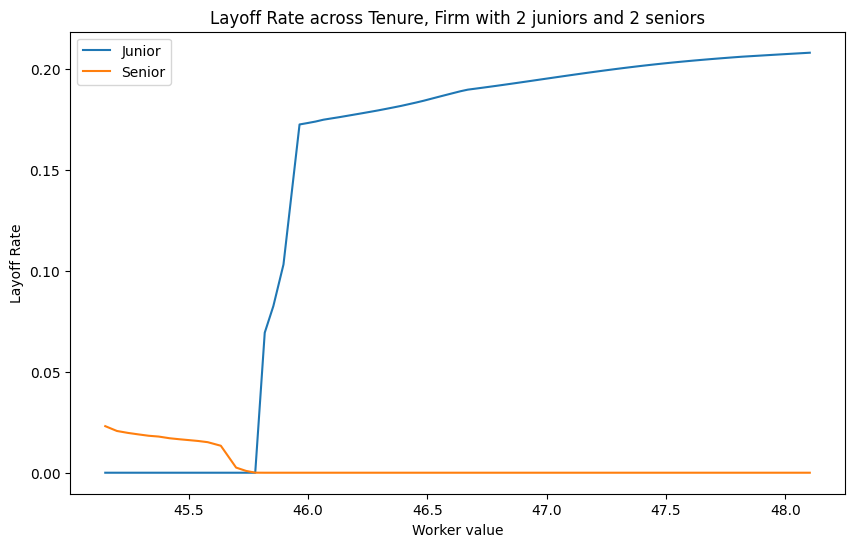
\includegraphics[width=0.7\textwidth]{Separations Across Tenure.png}
\end{frame}

\begin{frame}{Wage Cuts Smaller If Fire}
Simulate a single firm, no J2J transitions, force a negative prod shock. \\
\only<1-1>{
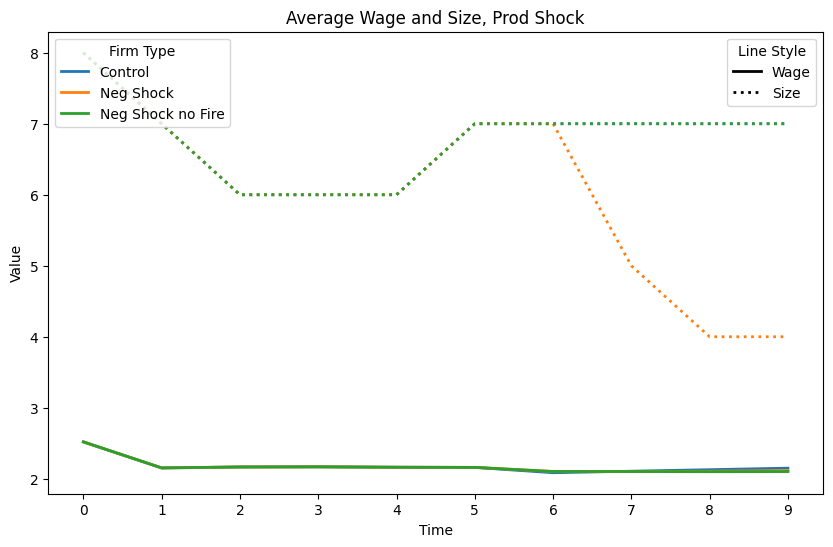
\includegraphics[width=0.65\textwidth]{Prod Shock Wages and Size.png}
}
\only<2-2>{
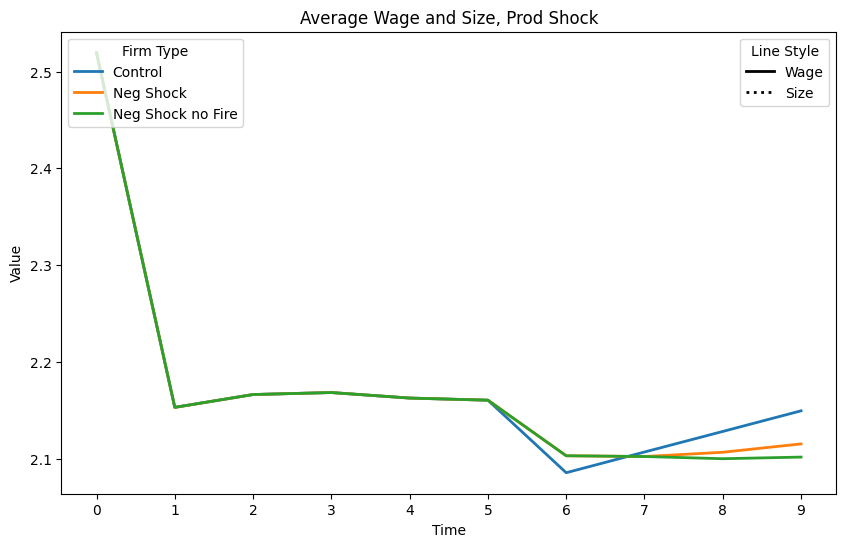
\includegraphics[width=0.65\textwidth]{Prod Shock Wages.png}
}
\\
Negative shock induces wage cuts, but the cuts are greater if not allowed to fire. \\
"Firms that report opportunistic layoffs are less likely to implement wage cuts" \textcolor{gray}{(Bertheau et al. 2024)}
\end{frame}

\begin{frame}{Empirical Validation: Firm's decisions across size}

Large firms have little productivity gain from extra workers $\rightarrow$ \textbf{fire} unproductive matches, mostly juniors \\
\only<1-1>{
\begin{figure}
    \centering
%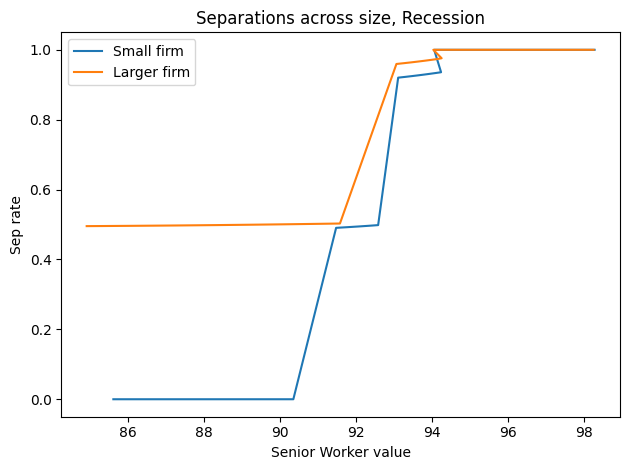
\includegraphics[width=0.4\textwidth]{Separations across size new.png} \\
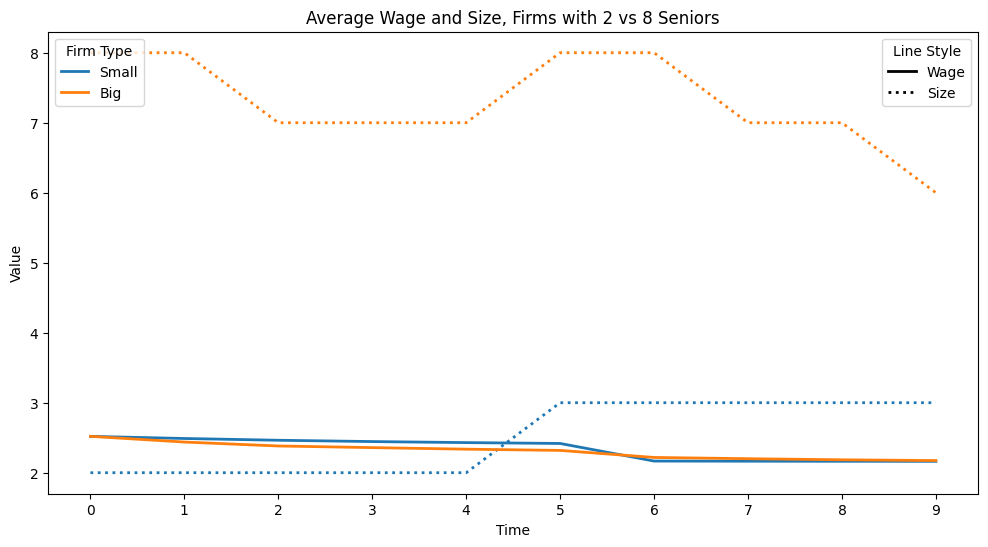
\includegraphics[width=0.7\textwidth]{Across Size Wages and Size.png}
\end{figure}
}
\only<2-2>{
\begin{figure}
    \centering
%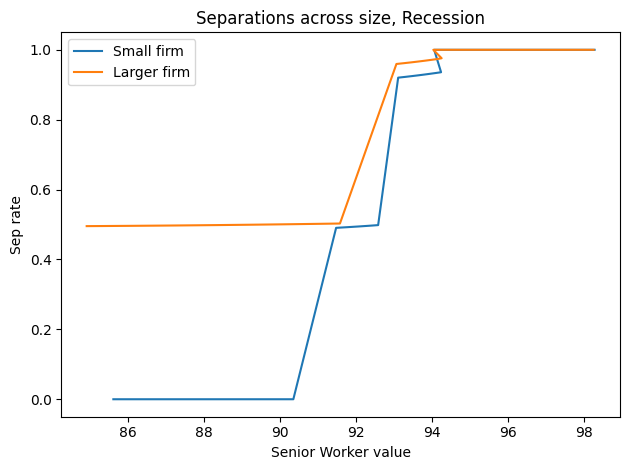
\includegraphics[width=0.4\textwidth]{Separations across size new.png} \\
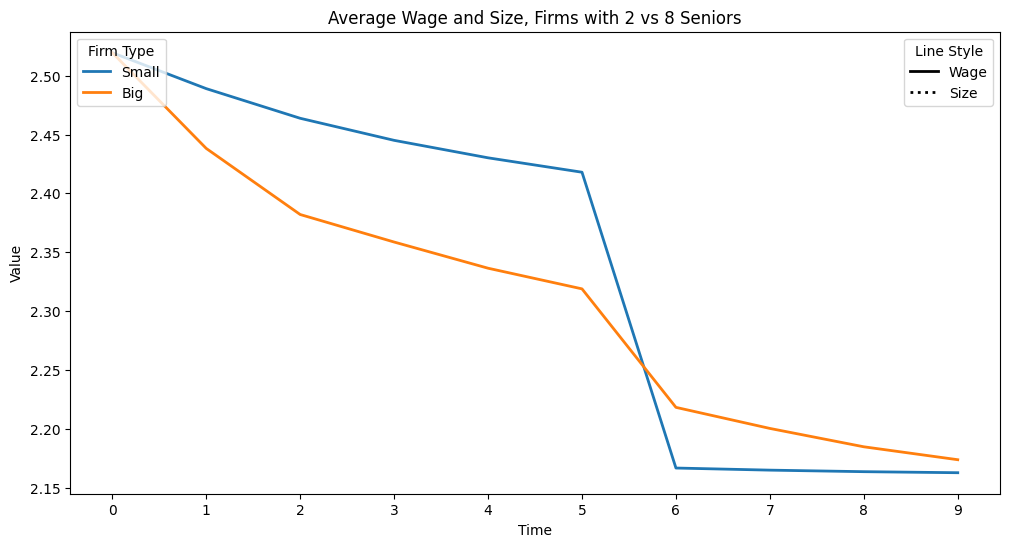
\includegraphics[width=0.7\textwidth]{Across Size wages.png}
\end{figure}
}
%\vspace{10pt}
\textbf{Testable prediction.} Controlling for firm productivity:
\begin{itemize}
    \item Large firms exhibit more cyclical layoffs, primarily of junior workers
    \item Small firms exhibit more cyclical wages
\end{itemize}
\end{frame}

\begin{frame}{Testing the implication in the data}
French Matched Employer-employee data DADS. \\
\midskip
Regress wages and layoffs on business-cycle proxy (unemployment), interacted with firm size and tenure
\vspace{20pt}
\[log(w_{ijt}) &= \sum_{s\in S}(\mu^s(t)+\alpha anc_{ijt}+\textcolor{cyan}{\beta^s} u_{rt}+\textcolor{orange}{\tilde{\beta}^s}anc_{ijt}u_{rt}) + \zeta x_{it} + FE_i + FE_j +\epsilon_{ijt}\]
\[s_{ijt} &= \sum_{s\in S}(\alpha anc_{ijt}+\textcolor{cyan}{\beta^s} u_{rt}+\textcolor{orange}{\tilde{\beta}^s}anc_{ijt}u_{rt}) + \zeta x_{it} +\epsilon_{ijt}\]
\smallskip
\begin{itemize}
    \item $\textcolor{cyan}{\beta^s}$ - cyclicality across firm size terciles
    \item $\textcolor{orange}{\tilde{\beta}^s}$ - interaction for worker tenure
\end{itemize}
\end{frame}

\begin{frame}{Testing the implication in the data}
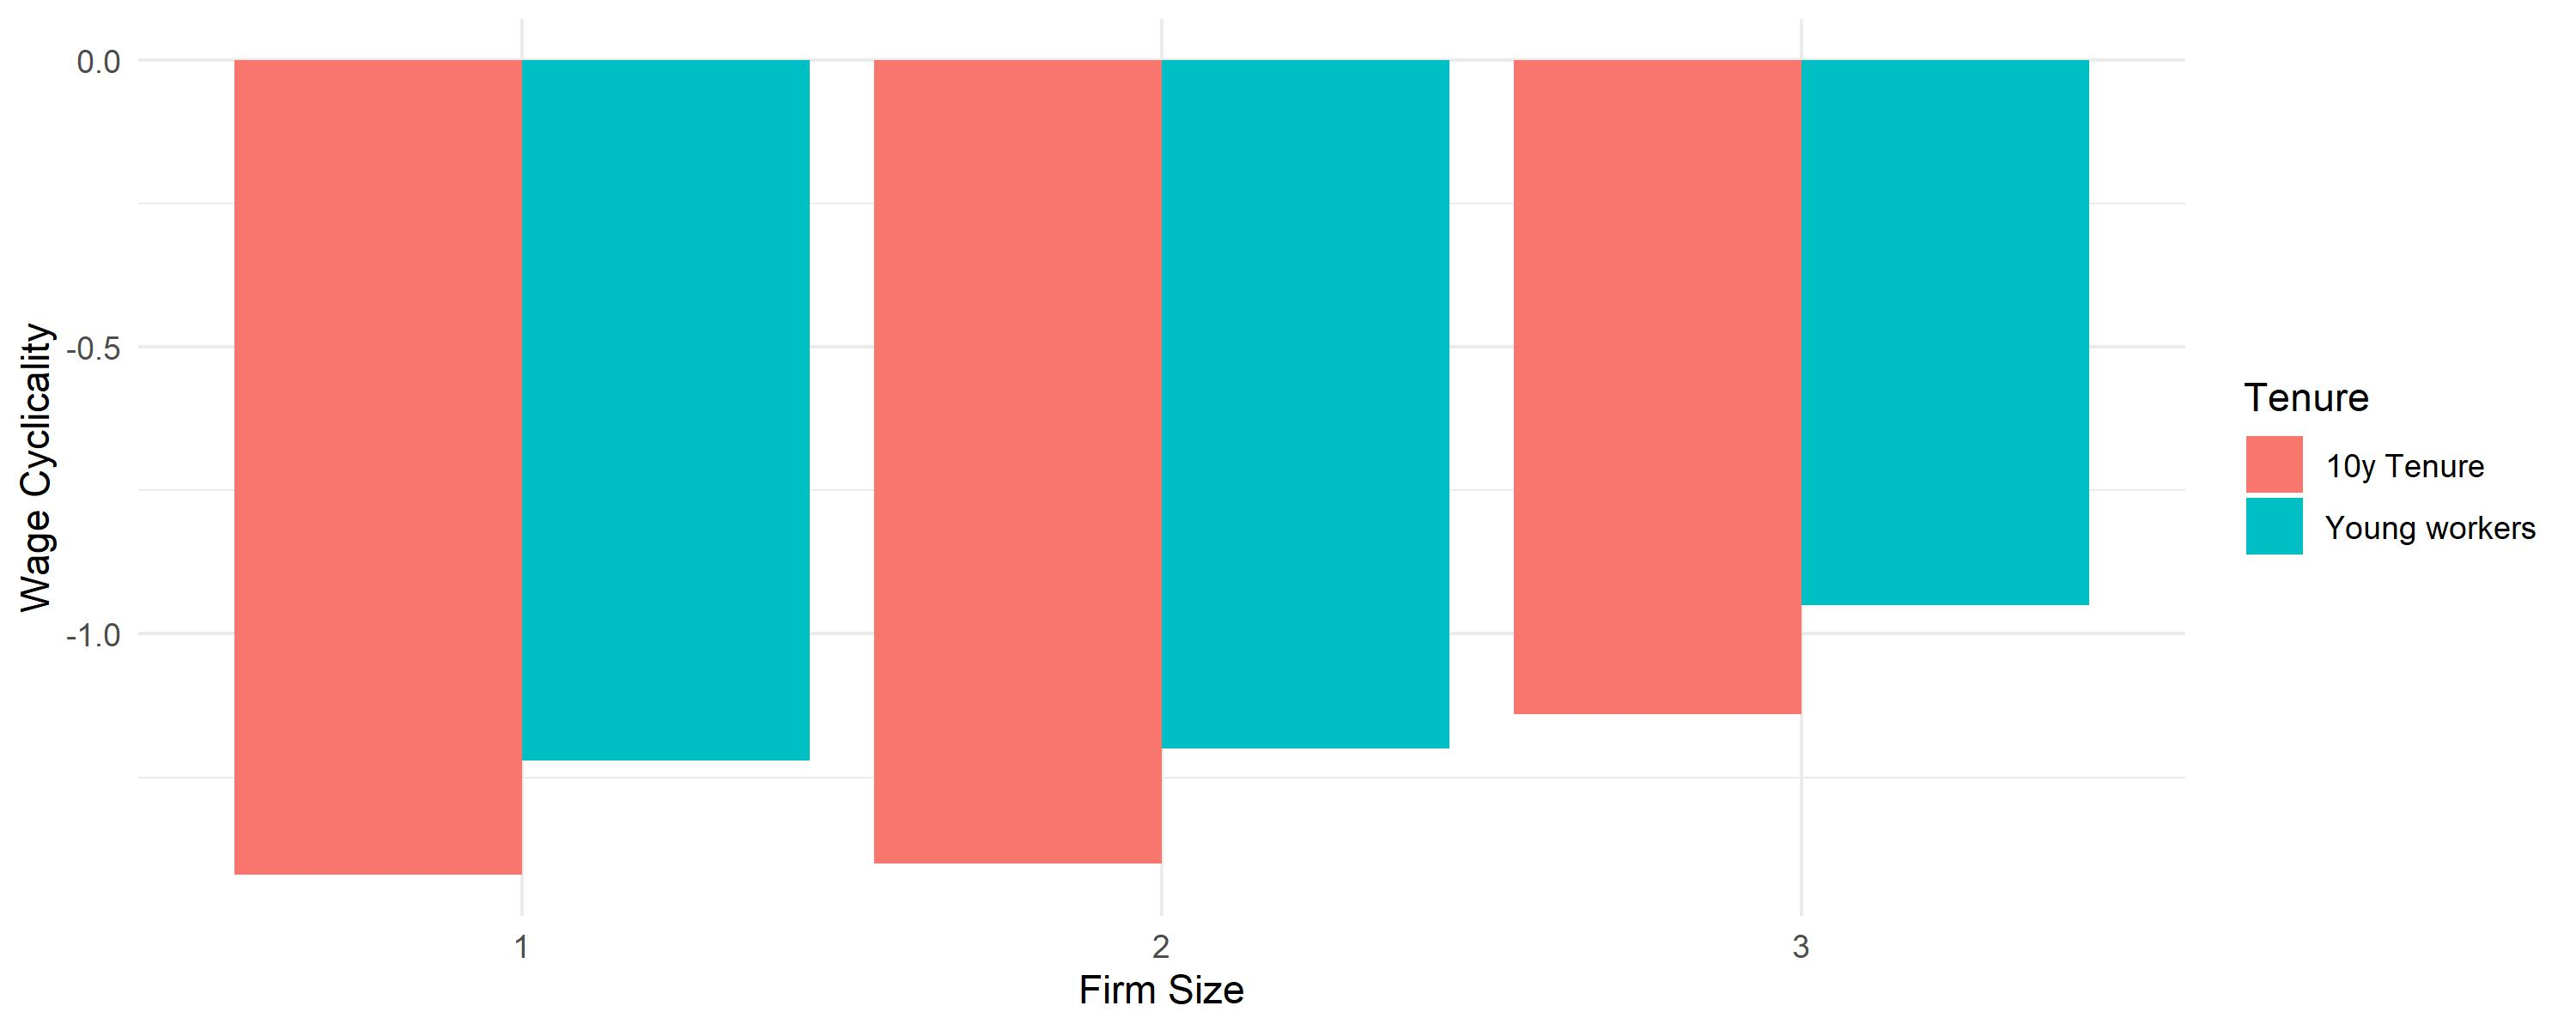
\includegraphics[width=0.95\textwidth]{Wage Cyclicality.jpg}
Smaller firms exhibit more cyclical wages \\
Tenured workers have more cyclical wages, uniformly across firms
\end{frame}

\begin{frame}{Testing the implication in the data}
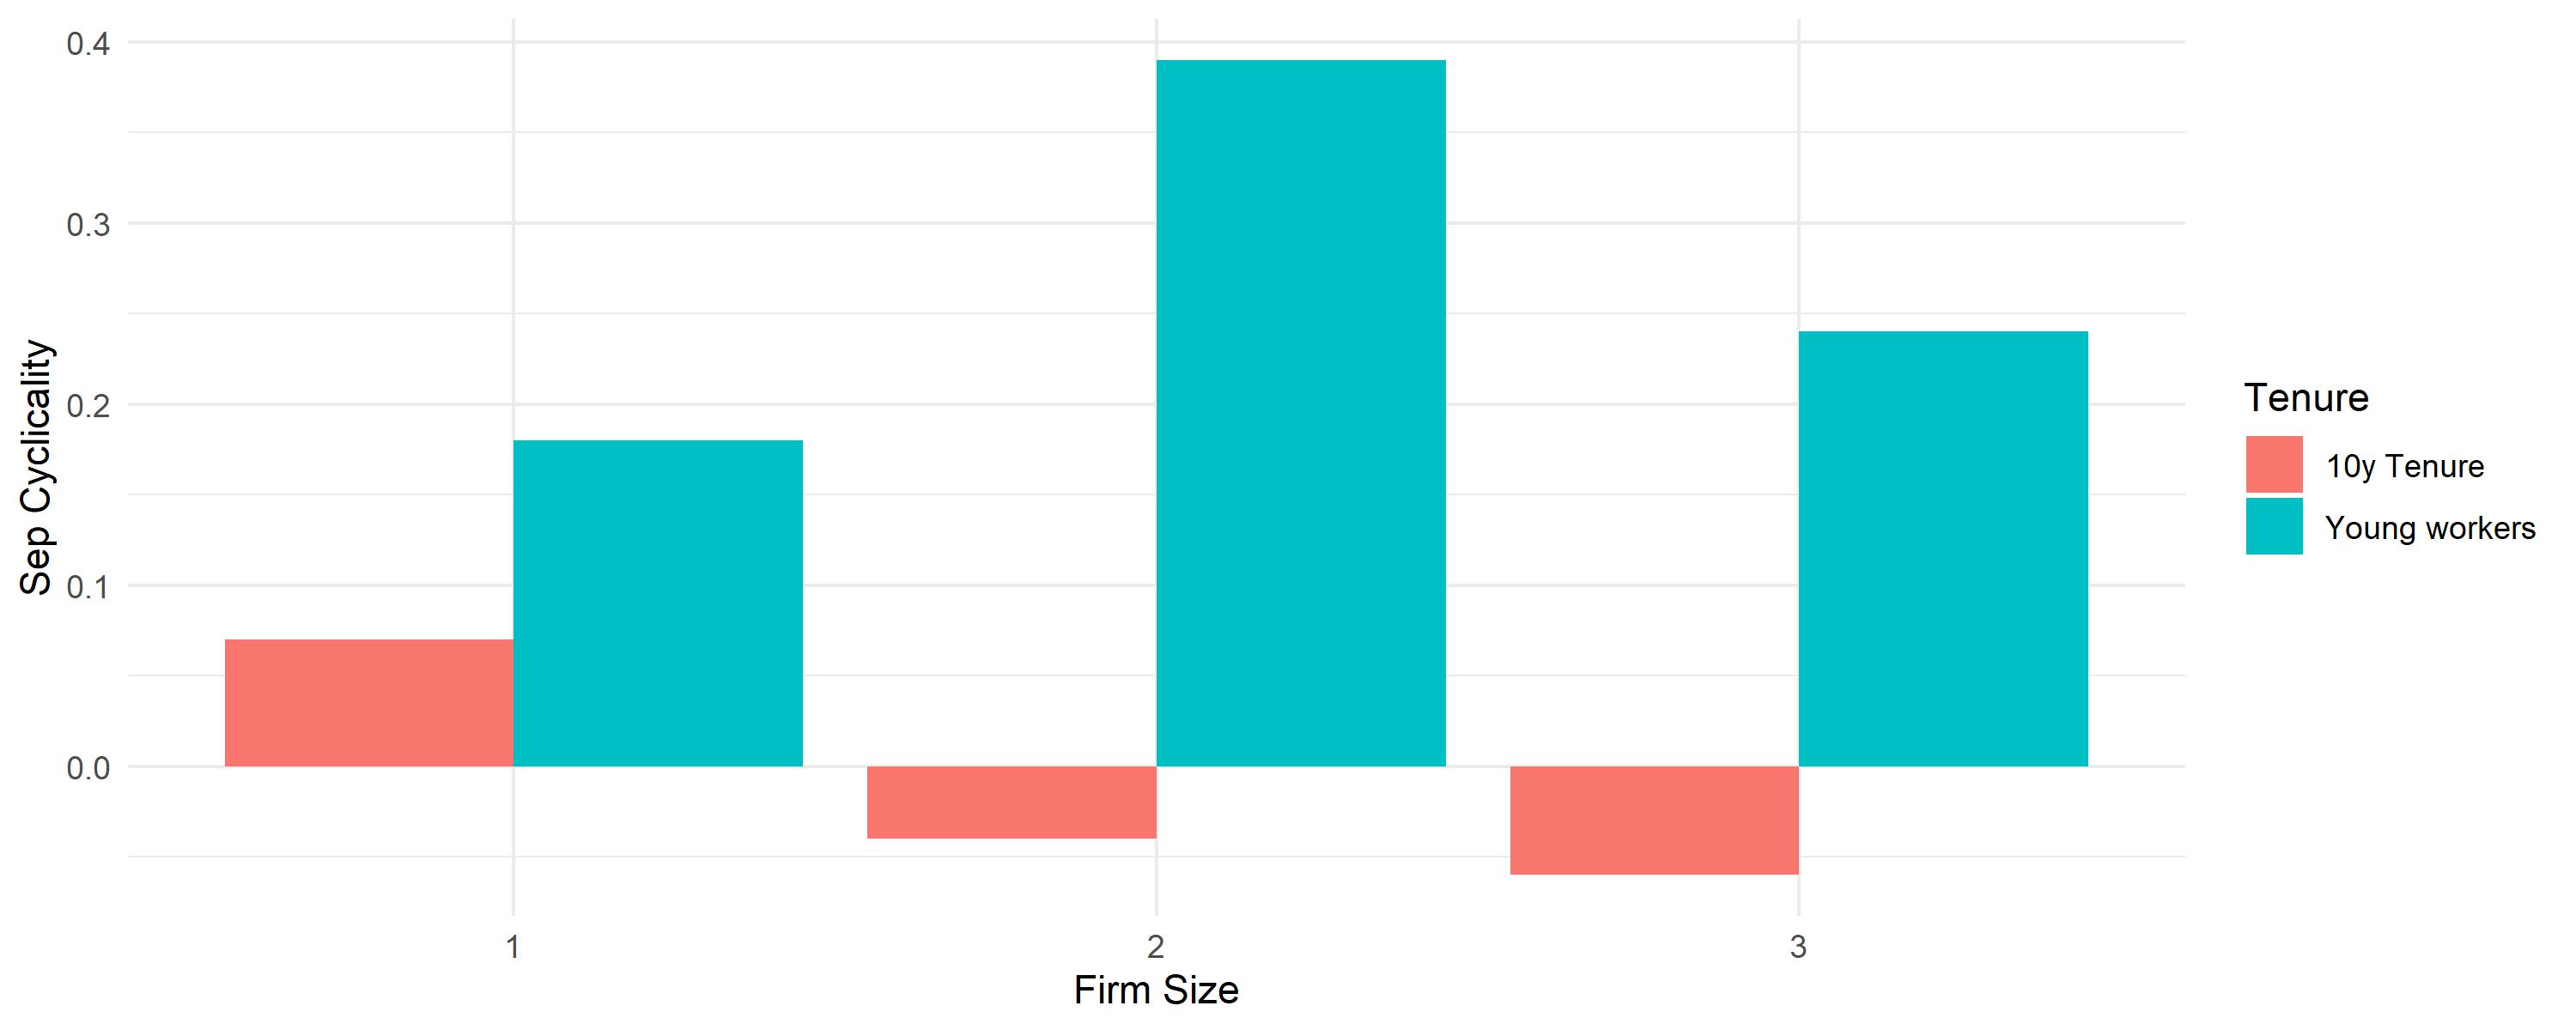
\includegraphics[width=0.95\textwidth]{Separations Cyclicality.jpg}
Larger firms exhibit more cyclical layoffs \\
Young workers have more cyclical layoffs, especially in larger firms \\
\textbf{Conclusion:} During negative shocks, small firms lower wages, while large firms fire young workers
\end{frame}

\begin{frame}{Conclusion}
\textbf{Puzzle:} Why are junior workers more subject to firings than wage cuts? \\
\bigskip
\textbf{Answer:} Juniors cheaper to fire, surviving juniors are of higher quality, so wage cuts less useful
\begin{itemize}
    \item Dynamic contracting in multi-worker firms with heterogeneous matches
    \item Endogenously generates layoffs
    \item Consistent with heterogeneity in wage and layoffs cyclicality across firm size and tenure
\end{itemize}
\bigskip
\textbf{To be done:}
\begin{itemize}
    \item Calibrate the model
    \smallskip
    \item Quantitatively reassess the motivating evidence
    \smallskip
    \item Consider policy implications
\end{itemize}
\end{frame}
%%%%%%%%%%%%%%%%%%%%%%%%%%%%%%%%%%%%%%%%%%%%%%%%%%%%%%%%%%%%
\begin{frame}[noframenumbering]{Motivating Evidence}
\hypertarget{MotivEv}
%Young workers are subject to higher than average aggregate earnings risk \textcolor{gray}{(Guvenen et al. 2017)} \\
%\begin{itemize}
%    \item At the firm level: Higher layoff rate, higher layoff passthrough, lower wage passthrough
%\end{itemize}
Young workers exhibit higher layoff risk, layoff passthrough, but lower wage passthrough. \\
All the age coefficients wash out after introducing tenure
\begin{table}
  \centering

  \label{tab:regression}
  \begin{tabular}{lcccccc}
    \hline
    & \multicolumn{4}{c}{Layoff rate} & \multicolumn{2}{c}{Log Wages} \\

    Regressors & (1) & (2) & (3) & (4) & (1) & (2) \\
    \hline
    Age                & $-0.16$ & $-0.04$ &     &                 &      & \\
\textcolor{red}{Tenure}             &         & $-0.45$ &                    &                  &        &  \\
    Firm Shock         &         &         & $-1.12$            & $-1.34$          & $-0.14$& $-0.35$ \\
    Firm Shock * Age   &         &         & $0.02$             & $-0.00$          & $0.10$ & $0.04$ \\
Firm Shock * \textcolor{red}{Tenure}&         &         &                    & $0.09$           &        & $0.22$ \\
    \hline
  \end{tabular}
  \caption{Layoffs and Wages passthrough across age and tenure. Time and experience (except (1),(2)) controls\footnote{Experience can play a similar role to tenure in disabling the effect of age in (1) and (2), but not in the passthrough regressions}. Worker and job FEs for wage regression. Data: DADS Panel + FARE, 2008-2019 \hyperlink{Intro}{\beamerbutton{Back}}} 
\end{table}

%Note: experience matters for the avg layoff risk, but not for the passthrough
\end{frame}

\begin{frame}[noframenumbering]{Related Literature}
\hypertarget{LTA}{}
\begin{itemize}
    \item \textbf{Separations puzzle:} Why do firms fire instead of lowering wages? \textcolor{gray}{Bewley (1998)} \\
    \underline{Contribution}: theory of separations based on optimal workforce management
\end{itemize}
\midskip
\begin{itemize}
    \item \textbf{Labor cleansing:} \textcolor{gray}{Davis and Haltiwanger (1990), Hall (2000), Berger (2018)} \\
     \underline{Contribution}: apply the theory to wage-separations trade-off
\end{itemize}
\pause
\bigskip
\begin{itemize}
    \item \textbf{Dynamic contracting with search frictions:} \textcolor{gray}{Balke and Lamadon (2022), Souchier (2023)} \\
\\
    \textbf{Firm dynamics with search frictions:}
    \textcolor{gray}{Elsby and Michaels (2013), Schaal (2017), McCrary (2022), Elsby and Gottfries (2022), Bilal, Engbom, Mongey, and Violante (2022)}  \\

   \underline{Contribution}: merge the two literatures
\\
    
\end{itemize}
\pause
    \bigskip
    \begin{itemize}
        \item \textbf{Technical contribution:} the two literatures combined not solvable in principle \\
        "A Limited Tenure Approximation” method allows to solve the model \underline{tractably} \\
 Wages flat in tenure after X years $\rightarrow$ enough to keep track of tenure at early stages of a career \hyperlink{Wage growth}{\beamerbutton{Wage growth in the data}}
    \end{itemize}
\end{frame}

\begin{frame}[noframenumbering]{Heterogeneous Match Quality}
\hypertarget{HMQ Assumption}{}

Consider a simplified, 2 period, contracting model. Assume completely persistent match types. \\
\[J(\{n_z\},v) = \max_{\{w_z\},\{w'_z\},\{s_z\},\{\tilde{s}_z\}} F(\{n_z\}) - \sum_{z} n_z w_z + \beta [F(\{n'_z\})-\sum_z n'_z w'_z]\]
s.t. LoM: \[n'_z = n_z (1-s_z)(1-p(w'_z))\] 
PK: \[u(w_z)+\beta[\tilde{s}_zU+(1-\tilde{s_z})((1-p(w'_z))u(w'_z)+p(w'_z)u(\hat{w})]=v\] 

In addition to this, firm may decide what kind of info to reveal to the worker.
\vspace{10pt}
\end{frame}

\begin{frame}[noframenumbering]{Heterogeneous Match Quality}
Assume: Firm is free to reveal information as long as it is not lying
\\
Assume additionally that the firm wants to keep high $z$ and lose low $z$ workers
\vspace{0.5cm}
\begin{itemize}
    \item Firm can get rid of low $z$ workers either by incentivizing OJS or firing them
    \vspace{5pt}
    \item \underline{Full information} reveal can help with OJS probability $p(w'_z)$
    \vspace{5pt}
    \item Firing is cheaper when information is \underline{not} fully revealed: high $z$ and low $z$ workers share the firing risk
    \vspace{5pt}
    \item Firm can utilize both at the same time: pool the low $z$ workers that it wants to fire with high $z$ ones
\end{itemize}
\vspace{0.5cm}
\textbf{Implcation:} Prevalence of layoffs depends on the likelihood of workers leaving during OJS $\rightarrow$ layoff more common in recessions, wage cuts - in more local shocks
\hyperlink{HMQ}{\beamerbutton{Back}} %\hyperlink{Reasons}{\beamerbutton{Details}} 
\end{frame}

\begin{frame}[noframenumbering]{Achieving Block Recursivity}
\hypertarget{Block Recur}{}
Assume all the jobs have the same starting value $v_0$
\begin{itemize}
    \item The choice of which submarket to post in does not affect the future value of the worker, just the sign-on bonus:
    \[min_{\tilde{v}}\Big[-\int_{v_0}^{\tilde{v}}\frac{1}{u'(w(v))}dv -\frac{c}{q(\theta(\tilde{v}))}\Big]\]
    where $w(v)$ such that $u(w(v))+\beta v_0=v$
    \item \textbf{Interpretation:} hires differ in their sign-on bonuses, not in their future wages
    \item This cost of hiring is independent of the firm's state
    \item Set $\theta(\tilde{v})$ such that \textbf{all} the firms are indifferent across \textbf{all} the submarkets
\end{itemize}
\vspace{5pt}
$\rightarrow$ Firms only care about productivity state, and \textbf{not} the distribution of labor
\hyperlink{PE}{\beamerbutton{Back}} 

\end{frame}

\begin{frame}[noframenumbering]{Full General Equilibrium}
\hypertarget{GE}{}
Fix the number of tenure steps $K$ in advance.
\vspace{5pt}
\begin{itemize}
    \item Each period, firms may enter the market upon paying a fixed cost $c$
    \item Upon entry, they start with a single worker at step $0$ and value $v_1$
    \item Free-entry condition at the firm-level: firms enter until $J(y_0,\{1,0,...\},\{v_1,...\})=c$
    \item Market tightness $\theta(v)$ is set such that 
    \begin{enumerate}
        \item New firms are indifferent between entering and staying out
        \item Incumbent firms are indifferent between hiring from different submarkets
    \end{enumerate}
    \item Once incumbent, firms treat $\theta$ as exogenous and solve the contracting problem. \hyperlink{PE}{\beamerbutton{Back}}

\end{itemize}
\end{frame}

\begin{frame}[noframenumbering]{Optimal Wage Growth in a Multi-worker Setting}
 \hypertarget{Wage K}{}
For every $1<k<K$, wage growth path nests that of a single-worker firm:
\[\frac{1}{u'(w'_{k})}-\frac{1}{u'(w_{k-1})}=\eta(v'_{k})\frac{\partial E_{y'|y}J'}{\partial n'_{k}}\]
The last promise $v'_K$ considers the effect on both upcoming and current long-term incumbents
\[\underbrace{\frac{1}{u'(w'_{K})}}_{\text{Costlier tomorrow}}-\underbrace{\frac{\frac{n_{K-1}(1-s_{K-1})}{u'(w_{K-1})}+\frac{n_{K}(1-s_{K})}{u'(w_{K})}}{n_{k-1}(1-s_{K-1})+n_K(1-s_K)}}_{\text{Both tenure levels cheaper today}}=\underbrace{\eta(v'_{K})\frac{\partial E_{y'|y}J'}{\partial n'_{K}}}_{\text{Higher retention probability}}\]
\hyperlink{Wage}{\beamerbutton{Back}}
\end{frame}

\begin{frame}[noframenumbering]{Firings without Heterog Match Quality}
\hypertarget{Sep}
If firms fire, they fire until
\[\underbrace{\frac{\partial E_{y'|y} J(y',{n'_k},\{v'_{y',k}\})}{\partial n'_{k}}(1-p(v'_k))}_{\text{Marginal benefit from losing a worker}}=\underbrace{\frac{U-R(v'_{k})}{u'(w_{k-1})}}_{\text{Compensation for firing risk}} \]
Firm still fires only if the worker brings negative profits. $\textbf{But}$:
\begin{itemize}
    \item Given a fixed number of steps, the firm is not completely free in choosing $v'_k$
    \vspace{2pt}
    \item Value of workers in step $K-1$ completely \textbf{tied} to those in $K$
    \vspace{2pt}
    \item During recessions, firm may decide to \textbf{fire} workers at step $K-1$ since it has no other way to (independently) lower their payrolls
\end{itemize}
\hyperlink{Hire}{\beamerbutton{Back}}
\end{frame}

\begin{frame}[noframenumbering]{Wage Growth across Tenure}
\hypertarget{Wage growth}{}
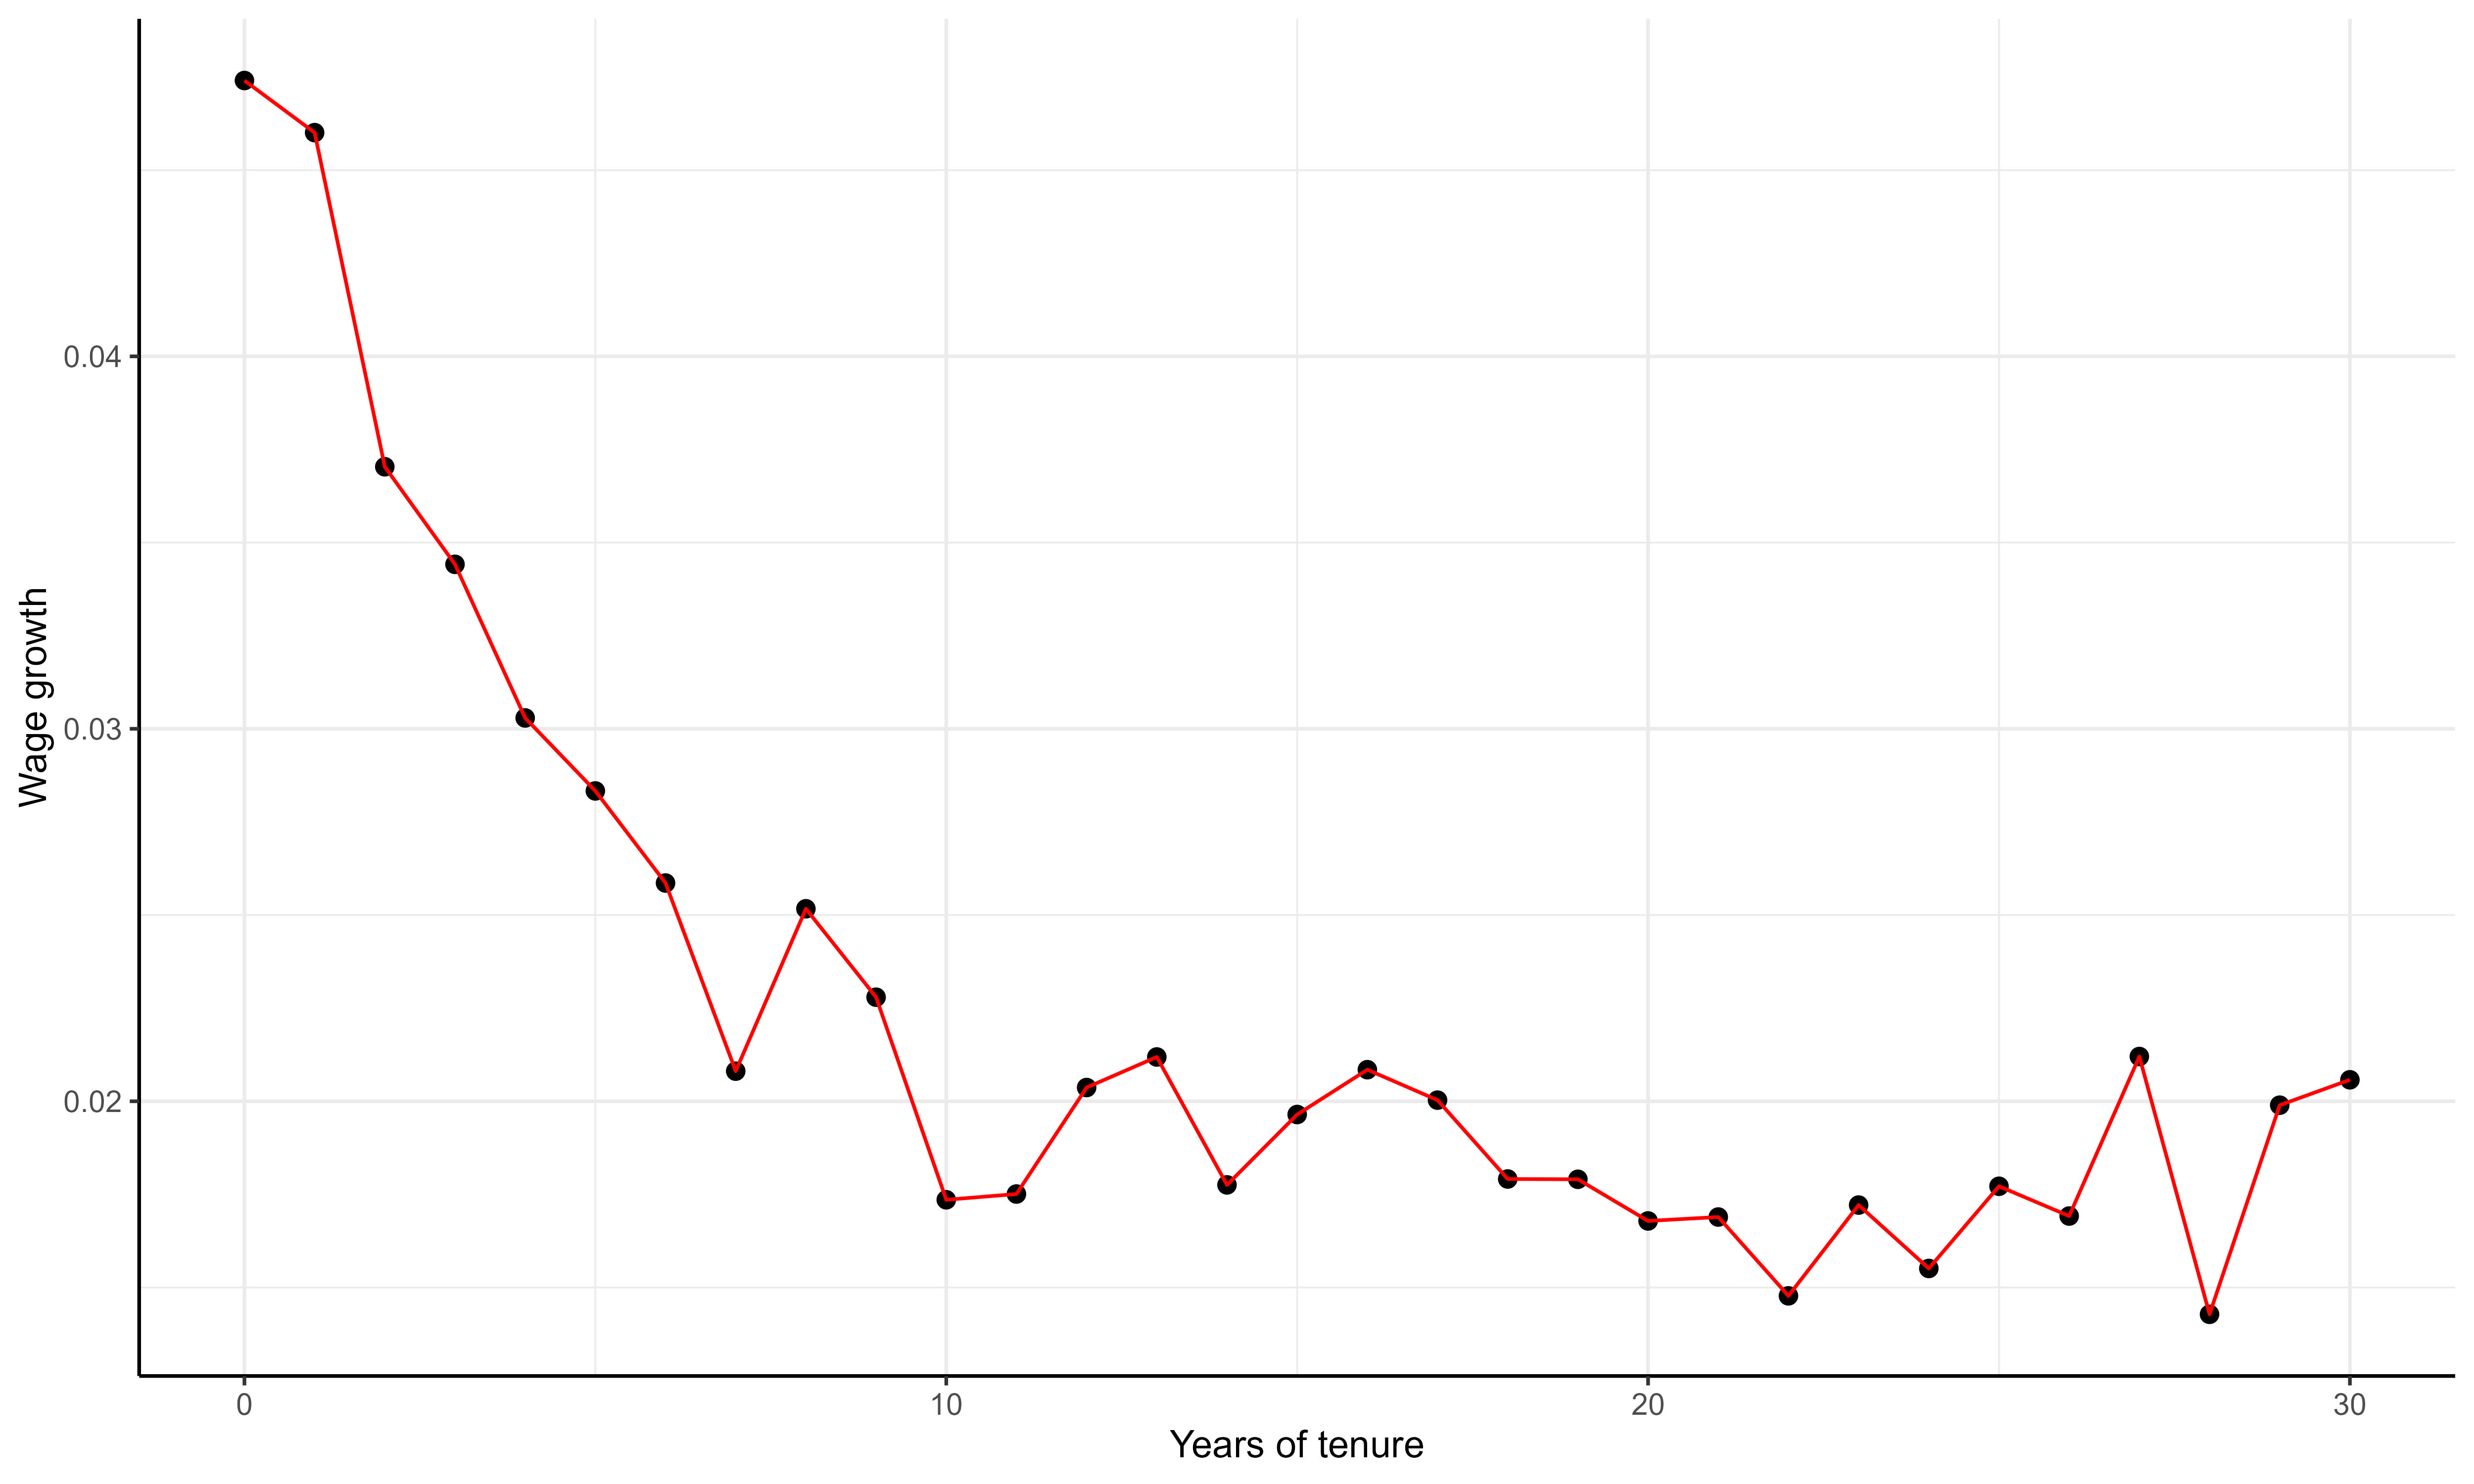
\includegraphics[width=0.75\textwidth]{Wage growth across tenure under 30,cutoff 100.jpg} \\
Log (real) wage growth appears to flatten after about 10 years of tenure at the firm.
\hyperlink{Contracting}{\beamerbutton{Back}}

\end{frame}
%%%%%%%%%%%%%%%%%CALIBRATION EXTRAS%%%%%%%%%%%%%%%%%%%%%%
\begin{frame}[noframenumbering]{Precise Parameters}
 \hypertarget{Calib}{}
\begin{itemize}
    \item Search function: hiring cost $\kappa$ (or match efficiency $\alpha$\footnote{Have to be careful, these are not isomorphic as in BL, might be better just to take Schaal's f-n, where he normalizies $\alpha=1$}), OJS search efficiency $s_{job}$
    \item Unemp production: $b$
    \item DRS: if curvature fixed\footnote{For curvature, can use employment share of $>500$ firms}, $\kappa_f$ and $\kappa_e$\footnote{Following Bilal et al. (2022), the latter may be directly pinpointed given other parameters. Not sure if applicable, but worth looking into}
    \item HMQ: ratio of good workers $q_0$ and relative prod-ty $p_q$
    \item Stoch prod-ty: correlation $\lambda_z$ and variance $\sigma_z$
    \begin{itemize}
        \item If I introduce agg prod-ty, need also the same for that + maybe correlation btw the two productivities?
    \end{itemize}
\end{itemize}
A total of 9 parameters + curvature of prod-n function
\end{frame}

\begin{frame}[noframenumbering]{Table of Moments}
    \begin{table}[h!]
\centering
\begin{tabular}{lccc}
\hline
Moments & Souchier/\textcolor{red}{Schaal} & Andrei \\
\hline
\hline
Average duration non-employed in months/Rate of new hires & 14.3 (0.063) &  12.8\%\\
\hline
Annual separation rate into non-employment & 5.5\% (0.071\%) & 4.3\% \\
\hline
Annual job-to-job transition rate & 6.6\% (0.10\%) & 6.3\% \\
\hline \hline
Tenure profile of wages at 7.5 years & 7.1\% (0.04\%) & 33\% \\

\hline \hline
s.d. of firm productivity growth & 0.30 (0.026) & 0.39 \\
\hline
s.d. of sector productivity growth & 0.057 (0.019) & 0.078 \\
\hline
Annual persistence of firm productivity & 0.81 (0.01) & 0.79 \\
\hline \hline
\textcolor{red}{Average estab size}/Firm size & 15.6& 17.9/32.5\\
\hline
\textcolor{red}{Ratio of jobs created by opening estab}/Opening firms & 21\% & 6\%\\
\hline
Proportion of jobs created by $>10/>100/>500$ firms &- & 0.87/0.59/0.38 \\
\hline \hline
National min to mean wage ratio & - &  0.44\\
\hline \hline 
\end{tabular}
\caption{Targeted moments in Souchier/Schaal vs. Andrei}

\end{table}
\hyperlink{Param}{\beamerbutton{Back}}
\end{frame}
\begin{frame}[noframenumbering]{HMQ Approaches}
Approach 1: Passthrough of productivity wrt separations ( interpretation 1pp increase in EU raises y by $x\%$) \\
Completely uncontrolled to include cross-section variation
\begin{itemize}
    \item Firm productivity: -... something
    \item Sect productivity: -0.046
    \item Agg productivity: 0.002
\end{itemize}
Approach 2: Response of senior/junior wage ratio to separations \\
Intuition: workers that survived layoffs are on avg higher quality, so should be better paid  \\
Use sd of wages across tenure levels within a firm/job+year to measure
\begin{itemize}
    \item Within a job
    \begin{itemize}
        \item Job FEs, so no cross-sectional variation: 1.88
        \item No job FEs: -0.85 
    \end{itemize}
    \item Within a firm
    \begin{itemize}
        \item Job FEs, so no cross-sectional variation: 1.24
        \item No job FEs: -1.94
    \end{itemize}
\end{itemize}
The intuition that seniors are better paid does not work on the cross-section, only across time. Why? Does it matter?
\end{frame}

\begin{frame}[noframenumbering]{HMQ Approaches}
Approach 3: Labor Share \\
When a firm fires, the total labor share of firm should go down, but the \textbf{per worker} share should go up, as the worse workers were fired \\
\begin{itemize}
    \item Per worker vs Total labor share response to EU without firm FE: 1.58/-0.37         
    \item Per worker vs Total labor share response to EU with firm FE: 0.04/0.10
\end{itemize}
Works only without firm FEs! Why? \\
Alternative: responses to productivity shocks.
\begin{itemize}
    \item Per worker vs Total labor share response to firm shock: -0.43/0.19
    \item Per worker vs Total labor share response to agg shock: -0.82/0.81
\end{itemize}
\textbf{DOES NOT} work when using hiring rate, even lagged
\begin{itemize}
    \item Per worker vs Total labor share response to hire rate without firm FE: 0.196/-0.002
    \item Per worker vs Total labor share response to hire rate with firm FE: 0.009/0.016
\end{itemize}
, but works exactly as expected with firm size: -0.022/0.018 \hyperlink{Param}{\beamerbutton{Back}}
\end{frame}

\end{document}



%%%%%%%%%%%%%%%%%%%%%%%%%%%%%%%%%%%%%%%%%%%%%%%%%%%%%%%%%%%%%%%%%%%%%%%%%%%%
\begin{frame}[noframenumbering]{Introduction}
\textbf{Puzzle:} Why do firms fire workers instead of lowering wages? \\
\smallskip
Without wage rigidity, existing models of firms/workers struggle to produce:
\begin{itemize}
    \item Large wage drops infrequent, firms prefer to fire
\end{itemize}
\textbf{Policy relevance:} does minimum wage amplify separations?  \midskip \\
Tentative explanation: firms use recessions as an opportunity to \textbf{restructure} (Kudlyak et al. 2023)\\
\bigskip
\pause
\textbf{This paper:}
\begin{itemize}
    \item \textbf{Dynamic contracts} in \textbf{DRS} firms with heterogeneous match quality
    \smallskip
    \item \textbf{Endogenously} generates separations without exog wage rigidity\\
    \smallskip
    \item Maps to heterogeneity in wage and separations cyclicality using \textbf{administrative French data}
\end{itemize}

\end{frame}

\begin{frame}{Related Literature}
Merge two literatures, with the same prediction: separate only if marginal worker is unproductive
\begin{itemize}
    \item \textbf{Dynamic contracting with search frictions:} \textcolor{gray}{Balke and Lamadon (2022), Souchier (2023)} \\
 
  \onslide<0>  Common prediction: adjust wage instead of firing (without extra assumptions) \\
   Contribution: separations can be generated endogenously in a multi-worker setting
    \\
    \vspace{5pt}
\onslide<1>   \item \textbf{Firm dynamics with search frictions:}
  \textcolor{gray}{Elsby and Michaels (2013), Schaal (2017), McCrary (2022), Elsby and Gottfries (2022), Bilal, Engbom, Mongey, and Violante (2022)}  \\
\onslide<0>  
  Common prediction: efficient wage and firm dynamics \\
  Contribution: separations even if the marginal worker generates surplus
\\
    
\end{itemize}
  
    \vspace{10pt}
    \textbf{What's more:} the two aspects combined not solvable in principle
    \begin{itemize}
        \item "A Limited Tenure Approximation” method allows to solve the model \textbf{tractably}
        \item Wages flat in tenure after X years $\rightarrow$ enough to keep track of tenure at early stages of a career
    \end{itemize} 
\end{frame}


\begin{frame}[noframenumbering]{Introduction: Version 1}
\textbf{Puzzle:} Why do firms fire workers instead of lowering wages? \\
\vspace{3pt}
Existing models of firms/workers struggle (rely on exogenous variations) to produce:
\begin{itemize}
    \item Large wage drops infrequent, firms prefer to fire
    \item Large firms fire more workers, mainly juniors, small firms lower wages
    %\item Wage adjustments frequent for smalls firms, larger firms rely more on extensive margins
    %\item The firing decision depends on the tenure of workers
    \item Firms use recessions as an opportunity to restructure (Kudlyak et al. 2023)
\end{itemize}
\vspace{5pt}
\pause
\textbf{This paper:}
\begin{itemize}
    \item \textbf{Dynamic contracts} in \textbf{multi-worker} firms with heterogeneous match quality
    \vspace{2pt}
    \item \textbf{Endogenously} generates the features above\\
    \vspace{2pt}
    \item Maps to the empirics using \textbf{administrative French data}
\end{itemize}

\end{frame}

\begin{frame}{Related Literature: Version 1}
Merge two literatures, with the same prediction: separate only if the marginal worker is productive
\begin{itemize}
    \item Dynamic contracting with search frictions: \onslide<0> \textcolor{gray}{Balke and Lamadon (2022), Souchier (2023)} \\
   \onslide<1>  
    Common prediction: adjust wage instead of firing (without extra assumptions) \\
   \textbf{Contribution:} separations can be generated endogenously in a multi-worker setting
    \\
    \vspace{5pt}
   \item Firm dynamics with search frictions: 
    \onslide<0> \textcolor{gray}{Elsby and Michaels (2013), Schaal (2017), McCrary (2022), Elsby and Gottfries (2022), Bilal, Engbom, Mongey, and Violante (2022)}  \\
  \onslide<1>   \\
  Common prediction: efficient wage and firm dynamics \\
  \textbf{Contribution:} separations even if the marginal worker is productive
\\
    
\end{itemize}
  
    \vspace{10pt}
    \textbf{What's more:} the two aspects combined not solvable in principle
    \begin{itemize}
        \item "A Limited Tenure Approximation” method allows to solve the model \textbf{tractably}
        \item Wages flat in tenure after X years $\rightarrow$ enough to keep track of tenure at early stages of a career
    \end{itemize} 
\end{frame}




\begin{frame}[noframenumbering]{Introduction: Version 2}
\textbf{Puzzle:} Why do firms fire workers instead of lowering wages? 
\begin{itemize}
    \item Survey evidence that firms use recessions as an opportunity to restructure (Kudlyak et al. 2023)\\
    \item Admin data evidence of heterogeneity in wages and separations across firm size and tenure
\end{itemize}
\vspace{5pt}
\pause
\textbf{This paper:} Dynamic contracting model in multi-worker firms with heterogeneous match quality
\begin{itemize}
    \item Not tractable in principle $\rightarrow$ made possible due to "Limited Tenure Approximation" method
\end{itemize}
\vspace{5pt}
\pause
\textbf{Mechanism:}
\begin{itemize}
    \item To maximize revenue, firms want both the highest quantity and quality of workers
    \item Recessions are perfect for the latter
    \begin{itemize}
        \item Marginal worker is less productive and cheaper to fire
    \end{itemize}
\end{itemize}
\textbf{Finding:} Large firms fire more workers, mainly juniors, small firms lower wages
\end{frame}

\begin{frame}{Related Literature: Version 2}
Merge two literatures:
\begin{itemize}
   \item Firm dynamics with search frictions: 
    \onslide<0> \textcolor{gray}{Elsby and Michaels (2013), Schaal (2017), McCrary (2022), Elsby and Gottfries (2022), Bilal, Engbom, Mongey, and Violante (2022)},  \\
  \onslide<1>   \textbf{Contribution:} Introduce contracting dynamics \\
  Allows to capture realistic wage dynamics of incumbent workers
  
    \vspace{5pt}
    \item Dynamic contracting with search frictions: \onslide<0> \textcolor{gray}{Balke and Lamadon (2022), Souchier (2023)} \\
   \onslide<1>  
    \textbf{Contribution:} Extend to a multi-worker firm setting \\
    Allows to capture effects of firm size and composition on wage dynamics
    \\
    \vspace{10pt}
    \textbf{Combining both:} can endogenously generate separation cyclicality and heterogeneity across firm size and tenure
\end{itemize}
\end{frame}

\begin{frame}

% Title at the top-center
\begin{center}
    \textbf{\huge Effects of}
\end{center}


% Place the terms semi-randomly in the middle section
\begin{textblock*}{3cm}(2cm, 1cm) % (x, y) coordinate for "Minimum wage"
    \begin{tikzpicture}
        \node {\Large \textbf{Minimum wage}};
        \draw[red, thick] circle[radius=1.3cm];
    \end{tikzpicture}
\end{textblock*}

\begin{textblock*}{4cm}(9cm, 0.8cm) % (x, y) coordinate for "Hiring subsidies"
    \begin{tikzpicture}
        \node {\Large \textbf{Hiring subsidies}};
        \draw[blue, thick] circle[radius=1.5cm];
    \end{tikzpicture}
\end{textblock*}

\begin{textblock*}{5cm}(5.5cm, 3cm) % (x, y) coordinate for "Short-term unemployment benefits"
    \begin{tikzpicture}
        \node {\Large \textbf{Short-term work}};
        \draw[teal, thick] circle[radius=1.45cm];
    \end{tikzpicture}
\end{textblock*}

\begin{textblock*}{5cm}(0.5cm, 3.7cm) % (x, y) coordinate for "Short-term unemployment benefits"
    \begin{tikzpicture}
        \node {\Large \textbf{Unemployment benefits}};
        \draw[green, thick] circle[radius=2.1cm];
    \end{tikzpicture}
\end{textblock*}

\begin{textblock*}{5cm}(10cm, 4.0cm) % (x, y) coordinate for "Severance payments"
    \begin{tikzpicture}
        \node {\Large \textbf{Severance payments}};
        \draw[orange, thick] circle[radius=1.8cm];
    \end{tikzpicture}
\end{textblock*}

% Text at the bottom-center
\begin{center}
    \vspace{7cm}
    \textbf{\huge depend on why firms fire their workers}
\end{center}

\end{frame}